\documentclass[aspectratio=169]{beamer}

\usetheme{Madrid}
\usecolortheme{seahorse}
\setbeamertemplate{navigation symbols}{}
\setbeamertemplate{footline}[frame number]

\usepackage{amsmath,amssymb}
\usepackage{booktabs}
\usepackage{graphicx}
\usepackage{xcolor}

\graphicspath{{paper_assets/}}

\newcommand{\E}{\mathbb{E}}
\newcommand{\Var}{\operatorname{Var}}
\newcommand{\norm}[1]{\left\lVert #1 \right\rVert}
\newcommand{\CV}{\operatorname{CV}}
\newcommand{\btheta}{\boldsymbol{\theta}}
\newcommand{\bbeta}{\boldsymbol{\beta}}

\title{Bayesian Rare State Detection in Crypto Markets}
\subtitle{Learning Which Data Matters for Scalable HMM Inference}
\author{Diego Luca Gonzalez Gauss, Enrico Yao-Bate, Haozhe Yang}
\institute{STAT 221 Spring 2026 Final Project}
\date{May 5, 2026}

\begin{document}

\begin{frame}
  \titlepage
\end{frame}

\begin{frame}{The data}
  \begin{itemize}
    \item \textbf{Assets:} daily spot returns for 5 crypto assets (BTC, ETH, SOL, BNB, AVAX) from Binance (quoted against USDT).
    \item \textbf{Period:} September 2020 - April 2026 ($\approx$2000 trading days) covering multiple market cycles, e.g. the 2021 bull run, 2022 crash (Terra/Luna, FTX), and 2024-25 recovery.
    \item \textbf{Preprocessing:} returns are rolling-standardized using a 30-day trailing window to remove low-frequency volatility drift and makes Gaussian emissions less misspecified.
    \item \textbf{Block structure:} the standardized series is partitioned into non-overlapping 10-day blocks ($N \approx 200$). For each block, we compute summary features (volatility, dispersion, tail counts, etc.)\ from the raw returns.
  \end{itemize}
\end{frame}

\begin{frame}{Why HMM?}
  \begin{columns}[T]
    \begin{column}{0.55\linewidth}
      Crypto assets go through extended periods of low volatility where daily returns are small and centered near zero. Then, abruptly, daily moves of 10-20\% become common, correlations spike, and drawdowns cascade across assets. We suspect these shifts are discrete, not gradual. An HMM captures this:
      \begin{itemize}
        \item Latent state $z_t \in \{1, \dots, K\}$: market regime.
        \item Return distribution depends on the regime:
        \[
          y_t \mid z_t=k \sim \mathcal{N}(\mu_k, \Sigma_k).
        \]
        \item Regimes tend to persist, i.e.\ if we are in calm today, we are likely in calm tomorrow:
        \[
          z_t \mid z_{t-1} \sim \operatorname{Categorical}(A_{z_{t-1},:}).
        \]
      \end{itemize}
    \end{column}
    \begin{column}{0.40\linewidth}
      \begin{block}{Example states}
        0: calm / low volatility.

        1: stressed / high volatility.
      \end{block}
    \end{column}
  \end{columns}
\end{frame}

\begin{frame}{Why MCMC?}
  We want the full posterior $p(z_t \mid y_{1:T}, \btheta)$ over model parameters and latent states. But it is complex because it is high-dimensional (transition matrix, emission parameters for each state) and involves discrete latent variables.

  \vspace{0.5em}
  \begin{itemize}
    \item EM gives a point estimate but no uncertainty quantification.
    \item Variational methods require choosing an approximating family, which can miss important posterior structure.
    \item MCMC targets the exact posterior.
  \end{itemize}

  \vspace{0.3em}
  \begin{block}{The problem}
    MCMC requires the full posterior gradient at every step. For an HMM, this means an $O(TK^2)$ forward-backward pass over the entire series. For long series, this is prohibitive.
  \end{block}
\end{frame}

\begin{frame}{Why stochastic-gradient MCMC?}
  The idea is that because the HMM log-posterior decomposes as a sum over time, instead of computing the full gradient, we can approximate it by sampling $M$ block indices $I_1, \dots, I_M$ from a distribution $p$ over the $B$ blocks, and reweighting by their sampling probabilities:
  \[
    \widehat G(\btheta)=
    \nabla\log p(\btheta)
    +
    \frac{1}{M}\sum_{m=1}^M
    \frac{g_{I_m}(\btheta)}{p_{I_m}},
    \qquad g_b(\btheta)=\nabla \ell_b(\btheta).
  \]

  SGLD update (Welling \& Teh, 2011):
  \[
    \btheta_{t+1} = \btheta_t + \frac{\eta_t}{2}\,\widehat{G}(\btheta_t) + \xi_t, \qquad \xi_t \sim \mathcal{N}(0, \eta_t\, I).
  \]
\end{frame}

\begin{frame}{Our main question: How do we set the block sampling distribution $p$?}  

  \vspace{0.8em}
  \normalsize
  A first-pass answer is uniform sampling $p_b = 1/B$ since it is unbiased and simple. However, it ignores the fact that not all blocks are equally informative. 
  
  \vspace{0.5em}
  In crypto, most blocks capture sideways price action, and only a few contain crashes, liquidation cascades, or regime transitions. These rare blocks carry most of the gradient signal for stress-regime parameters, meaning that if we consistently under-sample them, we may lose the ability to accurately detect when the market is entering or exiting a stress regime.

  \vspace{0.5em}
  \begin{block}{The statistical computing question}
    How should we set the block sampling distribution $p$ in SG-MCMC for HMMs to ensure rare but informative regimes are adequately represented in the gradient estimate?
  \end{block}
\end{frame}

\begin{frame}{An existing answer: TASS (Ou, Young, Sen, Dunson, 2024)}
  \begin{block}{Their answer}
    Sample each block in proportion to how much gradient signal it carries, so blocks that matter more for the posterior get sampled more often.
  \end{block}

  \vspace{0.3em}
  Formally, we want to choose sampling weights $a_n$ that minimize the variance of our stochastic gradient estimator $\E\|\widehat{\nabla} - \nabla\|^2$. If we knew the latent states $z_t$, we could compute each block's gradient contribution
  \[
    g_n(\btheta) = \sum_{t \in C_n} \nabla_{\btheta} \left[\log p(y_t \mid z_t) + \log p(z_t \mid z_{t-1})\right].
  \]
  and just as we set proposal weights proportional to the integrand in importance sampling, the variance-optimal thing to do here is to set block weights $a_n^\star$ proportional to gradient norms.

  \vspace{0.3em}
  \textbf{Problem:} these weights require knowing the latent states $z_t$, which are exactly what we are trying to infer, and the current parameter $\btheta$, which changes at every MCMC step.
\end{frame}

\begin{frame}{How TASS approximates optimal weights in practice}
  \begin{enumerate}
    \item \textbf{Cluster observations:} run $K$-means on $y_1, \ldots, y_T$ to get proxy state labels $\hat{z}_t$. 
    \item \textbf{Compute approximate block gradients:} evaluate the block gradient formula with $\hat{z}_t$ in place of $z_t$ and $\btheta$ fixed at $\btheta_{\mathrm{MAP}}$:
      \[
        \tilde{g}_n = \sum_{t \in C_n} \nabla_{\btheta} \left[\log p(y_t \mid \hat{z}_t) + \log p(\hat{z}_t \mid \hat{z}_{t-1})\right]\bigg|_{\btheta = \btheta_{\mathrm{MAP}}}.
      \]
    \item \textbf{Set weights:}
      $\displaystyle\tilde{a}_n = \frac{\norm{\tilde{g}_n}}{\sum_{n'=1}^{N}\norm{\tilde{g}_{n'}}}$ so blocks with many rare-state observations get large $\tilde{a}_n$.
    \item \textbf{Sample:} draw blocks with probabilities
      $\displaystyle p_n^{\mathrm{TASS}} = (1-\lambda)\,\tilde{a}_n + \frac{\lambda}{N},$ where the $\lambda/N$ is to ensure every block still has a chance to be sampled.
  \end{enumerate} 

  \vspace{0.3em}
  \begin{block}{Limitation}
    TASS weights are static. They only use emission values (through $K$-means), and cannot adapt if the importance of blocks shifts as the chain explores the posterior.
  \end{block}
\end{frame}

\begin{frame}{Our answer: learn which blocks matter during sampling}
    \begin{block}{High-level idea}
      Replace the static weights with a model that predicts each block's gradient importance from observable features, and updates those predictions during sampling using gradient feedback.
    \end{block}

  \vspace{0.5em}
  For each block $C_n$, we compute a feature vector $w_n \in \mathbb{R}^p$ from the observations in that block:
  \begin{itemize}
    \item mean absolute return, mean squared return,
    \item rolling volatility (within-block standard deviation),
    \item cross-sectional dispersion (spread across similar assets),
    \item tail event counts (number of returns exceeding a threshold),
    \item downside pressure (fraction of negative returns).
  \end{itemize}
  These are observable proxies for regime activity since stress blocks tend to have high volatility, large returns, and high dispersion.
\end{frame}

\begin{frame}{The online weight model}
  Recall from TASS that the optimal weight for block $n$ is $a_n^\star \propto \|g_n(\btheta)\|$. We want to predict this from the block features $w_n$, and update the prediction as $\btheta$ changes during sampling. 

  \vspace{0.5em}
  We opt to do this by turning it into a regression problem. Gradient norms are positive and vary over orders of magnitude, so we model the log-squared norm as linear in features:
  \[
    \log \norm{g_n(\btheta_t)}^2 \;\approx\; \widehat\bbeta_t^\top w_n,
  \]
  where $\widehat\bbeta_t \in \mathbb{R}^p$ is a coefficient vector, updated at each MCMC step $t$, that captures how each feature relates to gradient importance. This gives natural importance weight estimates
  \[
    \widehat a_{n,t} = \exp\!\bigl(\tfrac{1}{2}\,\widehat\bbeta_t^\top w_n\bigr) \;\approx\; \norm{g_n(\btheta_t)}.
  \]

  \vspace{0.5em}
  As in TASS, we convert weights to sampling probabilities with a uniform exploration floor:
  \[
    p_{n,t}
    =
    (1-\lambda)\,
    \frac{\widehat a_{n,t}}{\sum_{n'=1}^N \widehat a_{n',t}}
    +
    \frac{\lambda}{N}.
  \]
\end{frame}

\begin{frame}{Fitting $\widehat\bbeta_t$ by discounted ridge regression}
  At each SGLD step $t$, after sampling block $C_{n_s}$ and computing its gradient, we observe what we call the \textbf{feedback response} for our regression
  \[
    f_s = \log\bigl(\norm{g_{n_s}(\btheta_s)}^2 + \epsilon\bigr),
  \]
  which is just the regression target for block $n_s$, where $\epsilon > 0$ prevents $\log 0$.

  \vspace{0.3em}
  We need a regression method that (a) adapts to non-stationarity, since block importance shifts as $\btheta$ moves, and (b) has a cheap closed-form update, since it runs inside every SGLD step. Discounted ridge regression satisfies both, so we do
  \[
    \widehat\bbeta_t
    =
    \arg\min_{\bbeta}
    \sum_{s < t}
    \rho^{t-s}
    \bigl(f_s - \bbeta^\top w_{n_s}\bigr)^2
    +\tau\norm{\bbeta}^2,
  \]
  where the \textbf{discount} $\rho \in (0,1)$  down-weights old observations exponentially, so the model tracks shifting importance rather than averaging over the entire chain history, while our \textbf{ridge penalty} $\tau > 0$ regularizes early in the chain when few blocks have been sampled.

  \vspace{0.5em}
  This has a closed-form recursive update of $O(p^2)$ per step, so it is cheap enough to run inside every SGLD iteration.
\end{frame}

\begin{frame}{The full algorithm}
  \small
  \textbf{Input:} data $y_{1:T}$, blocks $\{C_n\}_{n=1}^N$ with buffer length $B$, features $\{w_n\}$, $\btheta_0$ from MAP
  \vspace{0.3em}
  \hrule
  \vspace{0.3em}
  \begin{enumerate}\setlength{\itemsep}{0.15em}
    \item[0.] Init ridge model: set $A = \tau I$, \; $\mathbf{b} = 0$, \; $\widehat\bbeta = 0$
    \item For $t = 1, \ldots, T_{\mathrm{iter}}$:
    \begin{enumerate}\setlength{\itemsep}{0.1em}
      \item[a.] \textbf{Weights:} if $t < T_w$, then $\;p_n = 1/N$; otherwise, compute $$\;\widehat a_n = \exp(\tfrac{1}{2}\widehat\bbeta^\top w_n), \quad p_n = (1\!-\!\lambda)\frac{\widehat a_n}{\sum_{n'}\widehat a_{n'}} + \frac{\lambda}{N}.$$
      \item[b.] \textbf{Sample:} draw $M$ block indices $I_1,\ldots,I_M \sim p$
      \item[c.] \textbf{Gradient:} for each $I_m$, compute buffered block gradient $g_{I_m}(\btheta_t)$ and then form $$\widehat G_t = \nabla\log p(\btheta_t) + \frac{1}{M}\sum_{m}\frac{g_{I_m}(\btheta_t)}{p_{I_m}}.$$
      \item[d.] \textbf{SGLD step:} update $\btheta_{t+1} = \btheta_t + \frac{\eta_t}{2}\widehat G_t + \mathcal{N}(0, \eta_t I)$
      \item[e.] \textbf{Ridge update:} for each $I_m$, compute $$f \!=\! \log(\|g_{I_m}\|^2 \!+\! \epsilon), \qquad A \!\leftarrow\! \rho A + w_{I_m}w_{I_m}^\top, \qquad \mathbf{b} \!\leftarrow\! \rho\,\mathbf{b} + w_{I_m}f, \qquad \widehat\bbeta \!=\! A^{-1}\mathbf{b}.$$
    \end{enumerate}
  \end{enumerate}
\end{frame}

\begin{frame}{Implementation details}
  \begin{itemize}
    \item \textbf{JAX autodiff:} the HMM forward pass is a sequence of matrix multiplications, which JAX differentiates automatically. This lets us compute $g_n(\btheta)$ for any block without hand-deriving gradients for emission or transition parameters.

    \item \textbf{Buffered block gradients:} cutting the series into blocks ignores the HMM's sequential dependencies at the boundaries since block $C_n$'s gradient depends on messages from neighboring blocks. To handle this, we flank each block with a buffer of $B$ observations on each side. The forward pass runs over the full buffered region, but \texttt{stop\_gradient} detaches the buffer so gradients flow only through the central block (Ma et al.\ 2017).

    \item \textbf{Gradient clipping:} block gradients are clipped at norm 2500 to prevent occasional extreme blocks from destabilizing the SGLD chain, especially in early iterations before step sizes have decayed.

    \item \textbf{4 parallel chains:} we run independent chains to compute $\hat{R}$ diagnostics, which is how we detect mixing failures in the results.
  \end{itemize}
\end{frame}


\begin{frame}{Does the algorithm recover known regimes?}
  To verify that our implementation is correct before applying it to real crypto data, we first tested on a 1D simulated HMM where the true stress periods are known. The image below shows the observed series with true stress states marked in orange.
  \begin{center}
    
\includegraphics[height=0.55\textheight]{simulated_univariate_recovery.pdf}
  \end{center}
  All three methods (uniform, TASS, online) recover the true stress periods, confirming that the SGLD sampler, block subsampling, and online weighting machinery all work as intended.
\end{frame}

\begin{frame}{Full HMM inference: $K=3$ collapses}
  Our original model was a $K=3$ (calm, stress, chaos) Student-$t$ HMM on raw returns. This failed because all three SG-MCMC methods assigned $>$99\% of observations to a single state, meaning the sampler never found the stress or crisis regimes we were looking for.

  \begin{center}
    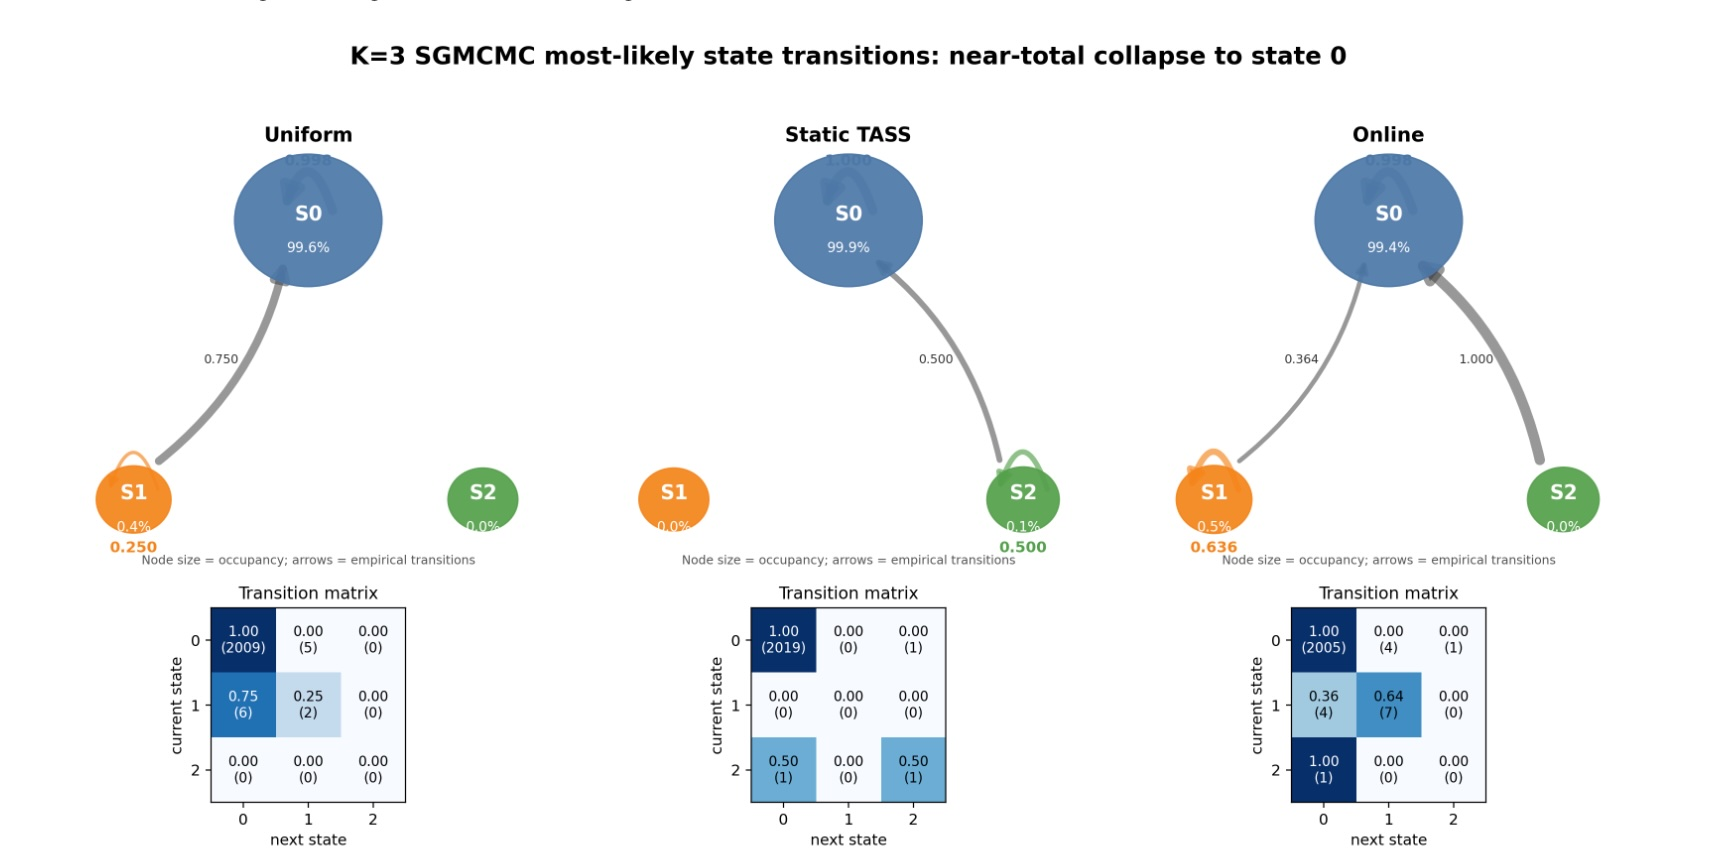
\includegraphics[height=0.42\textheight]{../IMG_0980.jpg}
  \end{center}
  \small Each panel shows the most-likely state transitions for one method. Node size is proportional to state occupancy; the transition matrices below confirm that states 1 and 2 are essentially empty. This is not just an SGLD problem because Stan/NUTS also failed for $K=3$ (max $\hat{R} = 2.21$, min ESS $= 5$), suggesting the third state is not identifiable from this data.
\end{frame}

\begin{frame}{Full HMM inference: $K=2$ on rolling-standardized returns}
  We simplified to $K=2$ Gaussian emissions on rolling-standardized returns. This gave interpretable regimes with roughly 60/40 calm vs.\ stress occupancy:
  \begin{center}
    
\includegraphics[height=0.48\textheight]{crypto_k2_state_probabilities.pdf}
  \end{center}
  \small The figure shows posterior stress-state probability over time for each method. Stan/NUTS mixes well for this model (max $\hat{R} = 1.04$, min ESS $= 48$), confirming it is identifiable.
\end{frame}

\begin{frame}{The mixing problem: SGLD chains do not converge}
  \begin{center}
    
\includegraphics[height=0.45\textheight]{sgmcmc_mixing_summary.pdf}
  \end{center}
  The figure shows $\hat{R}$ across parameters for each SGLD method on the $K\!=\!2$ crypto model. The standard convergence target is $\hat{R} < 1.05$ (Vehtari et al.\ 2021); all three methods remain above 2.0. Surprisngly, this persists even on simulated data where we know the ground truth.

  \vspace{0.3em}
  This suggests that the failures are not likely because of gradient variance, but because of the posterior geometry of the problem: label switching, transition/covariance coupling, and finite-step SGLD bias. And if so, better block weights cannot fix these structural problems.
\end{frame}

\begin{frame}{Isolating the mechanism: crypto stress prediction}
  To test online weighting where gradient variance \textit{is} the bottleneck, we built a simpler task that strips away HMM posterior geometry:

  \vspace{0.3em}
  \begin{block}{Forward-looking stress prediction}
    At the end of each 10-day block, predict whether the next 10-day equal-weight crypto basket return falls below $-7\%$:
    \[
      y_b = \mathbf{1}\{R_{b+1}^{\mathrm{mkt}} \le -0.07\}.
    \]
    We fit a ridge logistic regression with uniform / TASS / online.
  \end{block}

  \vspace{0.3em}
  The same math applies beacuse a few stress blocks carry most of the gradient signal, and observable features predict which blocks those are. But now there is no label switching, no multimodality, and no SGLD bias to confound the comparison.
\end{frame}

\begin{frame}{Does online weighting produce better risk forecasts?}
  \centering
  \resizebox{0.94\linewidth}{!}{\begin{tabular}{lrrrrrr}
\toprule
Method & Log loss & Brier & AUC & Top-risk stress rate & Strategy return & Max drawdown \\
\midrule
Online & 0.524 & 0.172 & 0.625 & 37.5\% & -33.3\% & -49.5\% \\
Static TASS & 0.531 & 0.175 & 0.623 & 25.0\% & -25.0\% & -48.3\% \\
Uniform & 0.533 & 0.176 & 0.620 & 25.0\% & -41.5\% & -55.1\% \\
Buy-and-hold & -- & -- & -- & -- & -49.7\% & -65.1\% \\
\bottomrule
\end{tabular}
}

  \vspace{0.8em}
  Yes. Online weighting outperforms both baselines on every calibration metric: best log loss (0.524), Brier score (0.172), and AUC (0.625). It also concentrates 37.5\% of actual stress events in the top-risk quartile, compared to 25\% for static TASS and uniform, meaning its risk scores are more informative about where stress actually occurs.
\end{frame}

\begin{frame}{What do the online risk scores look like?}
  \begin{center}
    
\includegraphics[width=0.92\linewidth]{actual_crypto_predicted_stress_probability.png}
  \end{center}
  The online model's predicted stress probability for each 10-day block. Spikes align with known crypto drawdowns (e.g.\ the May 2021 crash, Terra/Luna in June 2022, FTX in November 2022). The model learns to flag stress from observable features without being told which periods were stressful.
\end{frame}

\begin{frame}{Does online weighting actually reduce gradient variance?}
  To test this directly, we compute the true full gradient on real crypto data and compare the RMSE of each method's stochastic approximation.

  \vspace{0.5em}
  \centering
  \resizebox{0.7\linewidth}{!}{\begin{tabular}{lrr}
\toprule
Method & Mean RMSE & Top-decile sampling mass \\
\midrule
Oracle & 109.63 & 30.4\% \\
Online & 113.81 & 23.2\% \\
Static TASS & 117.39 & 24.6\% \\
Uniform & 132.99 & 10.0\% \\
\bottomrule
\end{tabular}
}

  \vspace{0.5em}
  \begin{itemize}
    \item Online achieves 14\% lower RMSE than uniform and 3\% lower than static TASS.
    \item Online is within 4\% of the oracle (which knows the true gradient norms).
    \item Online concentrates 23\% of sampling mass on the top-decile highest-gradient blocks (vs.\ 10\% for uniform).
  \end{itemize}
\end{frame}

\begin{frame}{What this tells us}
  \begin{block}{What worked}
    Online feature-informed weighting delivers on its core promise as a variance reduction tool: 14\% gradient RMSE improvement over uniform, 3\% over TASS, and the best downstream risk forecaster across all calibration metrics.
  \end{block}

  \begin{block}{What did not work}
    Full Bayesian HMM posterior inference via SGLD. The bottleneck turned out to be posterior geometry (label switching, weak identifiability of rare states, transition/covariance coupling, and finite-step SGLD bias) not gradient variance. Reducing gradient noise is necessary but not sufficient for reliable posterior sampling.
  \end{block}
\end{frame}

\begin{frame}{The lessons so far}
    \begin{itemize}
      \item Online weighting is most useful when block importance is heterogeneous, feature-predictable, and non-stationary. The stress prediction task satisfies all three.
      \item A Gaussian HMM on daily crypto returns may itself be a poor fit, since $K=3$ collapsed entirely, and even $K=2$ has posterior geometry that defeats SGLD. The model, not just the sampler, may need rethinking.
    \end{itemize}
\end{frame}

\begin{frame}{Next steps for the final paper}
  \textbf{Fixing the HMM inference:}
  \begin{itemize}
    \item Our prior of what constitutes a rare state may be wrong, so we should use stronger priors and explicit constraints on rare-state parameters.
    \item Marginalize the latent states $z_t$ analytically, reducing the posterior to continuous parameters and eliminating label switching.
    \item Explore different data granularities (hourly, weekly) which may change the regime structure and identifiability.
  \end{itemize}

  \vspace{0.3em}
  \textbf{Strengthening the online weighting theory:}
  \begin{itemize}
    \item Formal conditions under which online weighting improves convergence rates, not just gradient variance (connecting second-moment bounds to posterior convergence is open).
    \item Characterize when online provably beats TASS: how much drift in $\btheta$ is needed before static weights become stale?
  \end{itemize}
\end{frame}

\begin{frame}{References}
  \footnotesize
  \begin{itemize}
    \item Ou, R., Young, A. L., Sen, D., and Dunson, D. B. (2024). \textit{Targeted Stochastic Gradient MCMC for HMMs with Rare Latent States}. Bayesian Analysis.
    \item Welling, M. and Teh, Y. W. (2011). \textit{Bayesian Learning via Stochastic Gradient Langevin Dynamics}. ICML.
    \item Ma, Y., Chen, T., and Fox, E. (2017). \textit{A Complete Recipe for Stochastic Gradient MCMC}. NeurIPS.
    \item Vehtari, A., Gelman, A., Simpson, D., Carpenter, B., and B\"urkner, P.-C. (2021). \textit{Rank-normalization, folding, and localization: An improved $\hat{R}$}. Bayesian Analysis.
  \end{itemize}
\end{frame}

\end{document}
